\chapter{PCB Security basics}
A Printed Circuit Board(PCB) are objects that connect electronic, or not, devices together.
They are usually characterized by:
\begin{itemize}
  \item a non conductive support, that is usually 
  \item a mechanical robustness, meaning that is sturdy to mechanical modification(eg. bending)
  \item can connect electronical components
\end{itemize}
\begin{section}{PCB types}
  There are 3 main types of PCBs:
  \begin{itemize}
    \item Single sided PCBs, the simplest kind. It has one side to put components on and the other
      one for routing them.
    \item Double sided PCBs, in which components can be placed and routed on both sides, being more
      flexible than the single sided ones.
    \item Multi-layer PCBs, in which there are multiple layers in which the components can be placed
      and routed. They are the most complex and expensive kind of PCBs, but allows to partially
      ignore the space constraints of the other two kinds.
  \end{itemize}
\end{section}

\begin{section}{Materials and packages}
  Lets now talk for a second about what a PCB is made of. First of all, it has an insulating layer,
  usually made up of glass, with the Flame Retardant 4(FR4) being the most common. The metalization
  layer is usually made up of copper, and the components, which usually were through-hole, are now
  surface mounted, for example an SOP package.
  \begin{figure}[h]
    \centering
    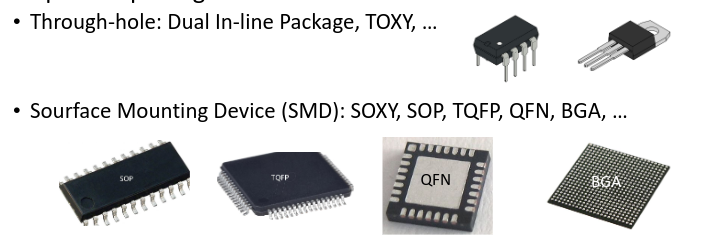
\includegraphics[width=0.5\textwidth]{img/hardware/pcp components.png}
    \caption{Some components of a PCB}
  \end{figure}
\end{section}
\\

A PCB can present different structures, like the one in figure \ref{fig:pcb-structure}. If you take
a look at the double sided one, you can notice that it has two copper layer to which the components
can be connected. Those can be connected in two ways: by vias, which are holes that connect the two
layers, or by traces, which are copper lines that connect the components. The second ones require no
metallization around the holes, being mostly used for mechanical components, whilst the first ones
require a metallization around the holes, being mostly used for electrical components.
\begin{figure}[h]
  \centering
  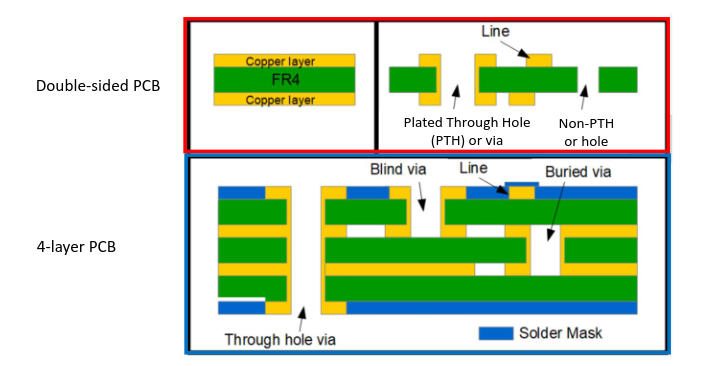
\includegraphics[width=0.7\textwidth]{img/hardware/pcb structure.png}
  \caption{A PCB structure}
  \label{fig:pcb-structure}
\end{figure}
The second example is more complex, being a multi-layer PCB. It has multiple layers, and the
components are connected by vias, which are holes that connect the different layers. The vias can
be of two types: blind vias, which connect the surface layer to the inner layer, and buried vias,
which connect two inner layers. The vias can be filled with a conductive material, like copper, to
improve the connection between the layers.

\begin{section}{Design flow}
  To design a PCB, we must first need to know what to to, and then we can start the design flow by
  using some kind of tools, like Altium Designer, KiCad, or Eagle. The first step is to know exactly
  the footprint of the components, because different components have different footprint, like the
  pin number, the pitch, the size, and so on. This is necessary to know how to place the components
  on the PCB. The second step is to enter the PCB size and design rules in the software, like the 
  minimum trace width. After that, we can start placing the components on the PCB, and then we can 
  start routing them. The last step is to generate the Gerber files, which are the ascii files that
  the manufacturer will use to produce the PCB.
\end{section}

\begin{section}{Security issues}
  Of course, we would like to have a secure board returned by the manufacturer. A trusted supply
  chain is good but not sufficient, in fact one of the biggest issues is to have no leakage of
  information from the integrated circuit, to avoid reverse engineering. At this day, most of PCB
  design have no protection, meaning that any user can try to probe and tamper the board.\\ 
  A board use standard communication protocols, to internal or external communications, and those
  increase the interruptibility of the board, and those can be exploited to extract informations,
  since the protocols are well known. Some of those protocols are:
  \begin{itemize}
    \item I2C
    \item SPI
    \item UART
    \item JTAG
  \end{itemize}
\end{section}

\begin{section}{Serial and parallel transmission}

  To try to understand why interrupts can allow the leakage of information, we need to understand
  how the data is transmitted. There are two main ways to transmit data: serial and parallel.
  Serial transmission protocols are used to transmit data one bit at a time, in a sequential order,
  whilst parallel transmission protocols are used to transmit data multiple bits at a time, carried
  by multiple wires. 
  \begin{figure}[H]
    \centering
    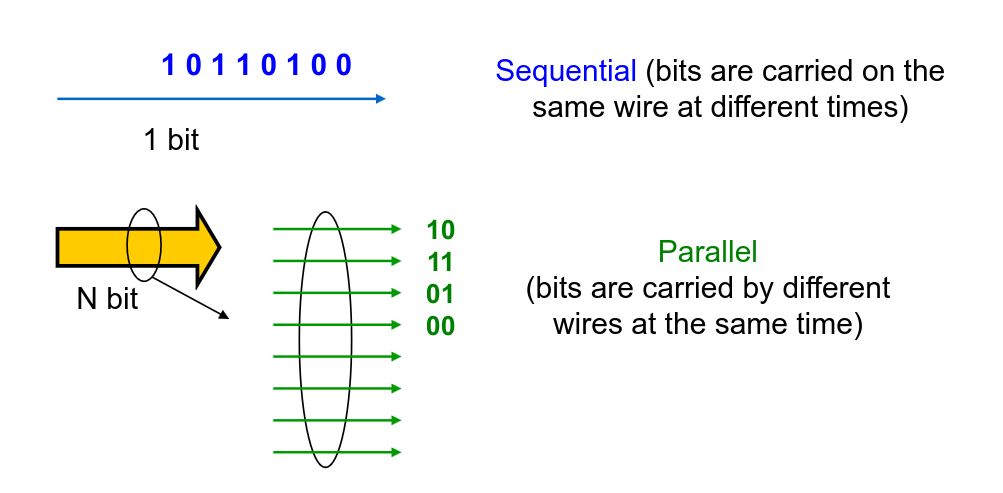
\includegraphics[width=0.5\textwidth]{img/hardware/pcb data transmission.png}
    \caption{Serial vs parallel transmission}
  \end{figure}
  \begin{subsection}{Serial Links}
    Serial links are very used because they are cheaper and easier to implement, requiring less wires 
    and less space, but they have a very high latency: to transmit $N$ bits, we need $N$ transfer
    cycles. Think kind of link is ideal for low throughput connections.\\
    Since the serial communication protocol is pretty simple, the general structure of a serial link
    is well defined, as shown in figure \ref{fig:serial-link}. At the trasmitter side, we have a 
    parallel-in-serial-out(PISO) shift register, which is filled with the data to be transmitted,
    and then sent one bit at a time to the receiver. At the receiver side, we have a
    serial-in-parallel-out(SIPO) shift register, where the bits are received one clock cycle at a time.
    The time needed to trasmitt one bit is usually called bit period, or duration, and as a
    consequence the bit rate is the reciprocal of the bit period($\text{Bit Rate} =
    \dfrac{1}{T_{\text{bit}}}$).\\
    Before the data is sent, a preamble is needed to synchronize the transmitter and the receiver,
    and a closure is needed to signal the end of the transmission. 
    \begin{figure}[H]
      \centering
      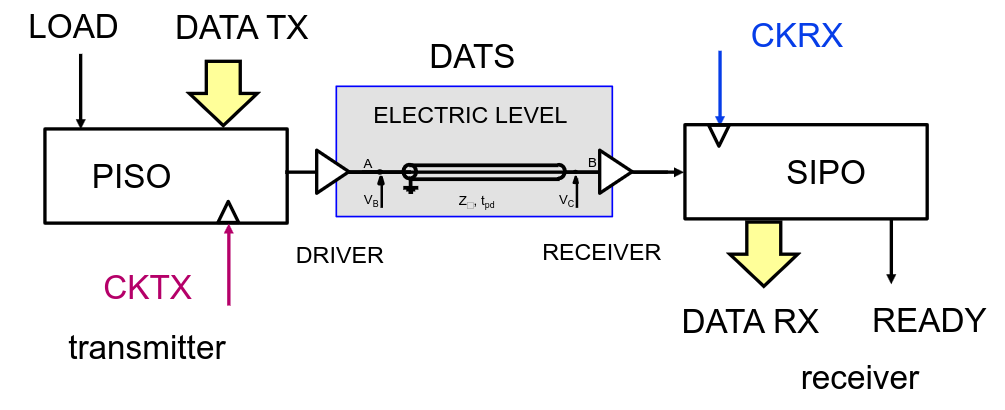
\includegraphics[width=0.7\textwidth]{img/hardware/serial link.png}
      \caption{Serial link structure}
      \label{fig:serial-link}
    \end{figure}
    The transmission can be synchronous or asynchronous. In the first case, the clock is shared, so
    a link to transmit it is needed, whilst in the second case it is not needed.\\
  \end{subsection}

  Another distinction can be made based on the direction of the data flow: simplex, half-duplex, and 
  full-duplex. In the first case, the data can flow only in one direction, whilst in the second case
  the data can flow in both directions, but not at the same time. In the last case, the data can
  flow in both directions at the same time.
\end{section}

\begin{section}{Serial Communication Protocols}
  \begin{subsection}{Serial Asynchronous Protocols}
    Since the protocol is asynchronous, only one link is needed. First of all the resting state is
    the logic high level, meaning that when the data is is being trasmitted, the beginning
    character is signaled by a logic low level, called start bit. To signal that the communication
    is over, the channel is kept at a logic 1 for a certain amount of time(the bit time), called
    stop bit. 

    \begin{figure}[H]
      \centering
      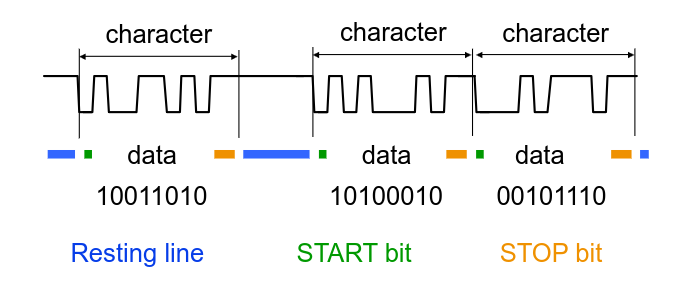
\includegraphics[width=0.7\textwidth]{img/hardware/serial asybncronous transmission.png}
      \caption{Serial asynchronous transmission}
    \end{figure}
    \begin{subsubsection}{UART}
      The trasmission with UART is asynchronous, so the data is loaded in the PISO register, and
      then sent one bit at a time. The receiver receives the bits one at a time, and then loads
      them in the SIPO register. Some logic to detect a transmission is needed, and some additional
      one can be added to perform some error checking(eg. parity bit).
    \end{subsubsection}
  \end{subsection}

  \begin{subsection}{Serial Synchronous Protocols}
    Other examples of serial communication protocols are synchronous, meaning that a clock is needed
    to synchronize the transmitter and the receiver. 
    \begin{subsubsection}{I2C}
      The I2C protocol is the most common and simple synchronous protocol. It has two wires, one for 
      the clock(Serial Clock Line,SCL) and one for the data(Serial Data Line,SDA). This means that
      only half-duplex communication is possible. It can also run up to 1MHz.\\
      The system stays in a idle state when both the SCL and the SDL are high. When a communication
      is starting, a SDA commutation is made when the SCL is low.

      \begin{figure}[H]
        \centering
        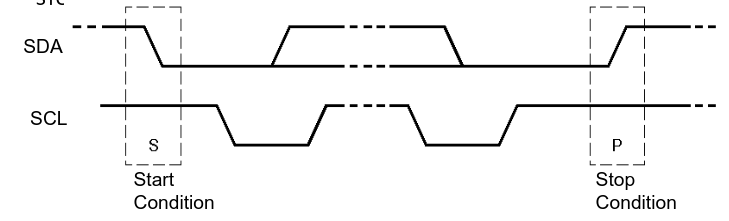
\includegraphics[width=0.5\textwidth]{img/hardware/ic2 commutation.png}
        \caption{I2C commutation}
      \end{figure}
      The transmission is byte oriented, meaning that an acknowledgment is needed after each byte,
      transmitted on the SDA line. One of the issues that have to be addresed are which slave we
      want to communicate to, so the first 7 bits are the address of the slave, and the last bit is
      the read/write bit(1 for reading and 0 for writing). The slave then sends an acknowledgment
      bit if it was able to detect it's own address on the SDA line. If the SDA line is low, the
      slave is ready to enstablish the communication, otherwise the line stays high.\\
      \begin{figure}[H]
        \centering
        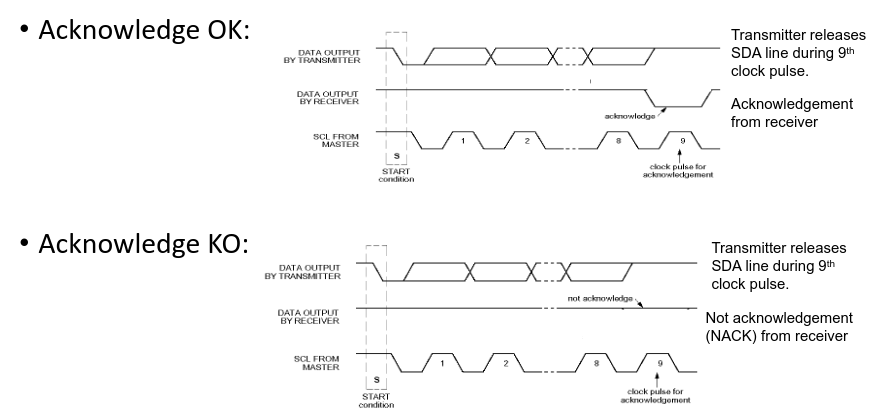
\includegraphics[width=0.7\textwidth]{img/hardware/ic2 ack.png}
        \caption{The acknowledgment process of the I2C protocol}
      \end{figure}

      \begin{figure}[H]
        \centering
        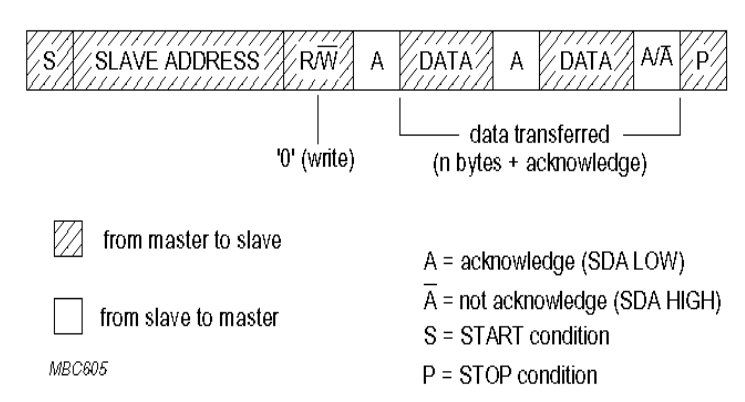
\includegraphics[width=0.5\textwidth]{img/hardware/i2c summary.png}
        \caption{Summary of the transmission from the master to the slave in the I2C protocol}
      \end{figure}
      Probing this kind of communication is very simple, because the channel is well defined.
    \end{subsubsection}
    
    \begin{subsubsection}{SPI}
      The SPI protocol is a synchronous protocol that uses 4 wires: one for the clock, one for the
      data, one for the master to select the slave, and one for the slave to signal that it is ready.
      This means that full-duplex communication is possible, allowing up to 10 MHz of communication.
      The general connection from a master to a slave is shown in figure \ref{fig:spi-connection}.
      The clock is always provided by the master, and the data flows via the MOSI(Master Out Slave
      In) and MISO(Master In Slave Out) lines.\\

      \begin{figure}[H]
        \centering
        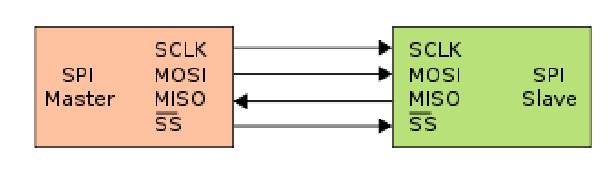
\includegraphics[width=0.5\textwidth]{img/hardware/spi connection.png}
        \caption{Example of SPI connection}
        \label{fig:spi-connection}
      \end{figure}
      The master selects the slave by pulling the SS line low, and the slave signals that it is
      ready by pulling the MISO line low. The unselected slaves keep the MISO line high.\\
      The standard configuration is not very scalable, because it requires lots of line( 1 ss line 
      for each slave), so an alternative configuration is the daisy chain configuration, shown in
      figure \ref{fig:spi-daisy-chain}. In this configuration, the data is passed from one slave to 
      the other, meaning that each slave has to be able to detect if the data is for it or not.
      \begin{figure}[H]
        \centering
        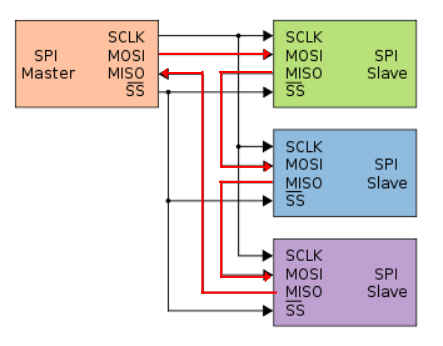
\includegraphics[width=0.5\textwidth]{img/hardware/spi daisy chain.png}
        \caption{SPI daisy chain configuration}
        \label{fig:spi-daisy-chain}
      \end{figure}
    \end{subsubsection}

    \begin{subsubsection}{JTAG}
      The JTAG protocol is a synchronous protocol usually used for debugging microcontroller. It
      implements a TAP(Test Access Port) used for controlling and configuring the device, which is
      made of 3 parts:
      \begin{itemize}
        \item A small finite state machine(FSM) that controls the TAP
        \item A set of registers that can be accessed by the TAP
        \item A set of instructions that can be executed by the TAP
      \end{itemize}

      The standards specifies 4 signals: TCK, TMS, TDI, and TDO. The first one is the clock, the
      second one is the mode select, the third one is the data input, and the last one is the data
      output. 

      \begin{figure}[H]
        \centering
        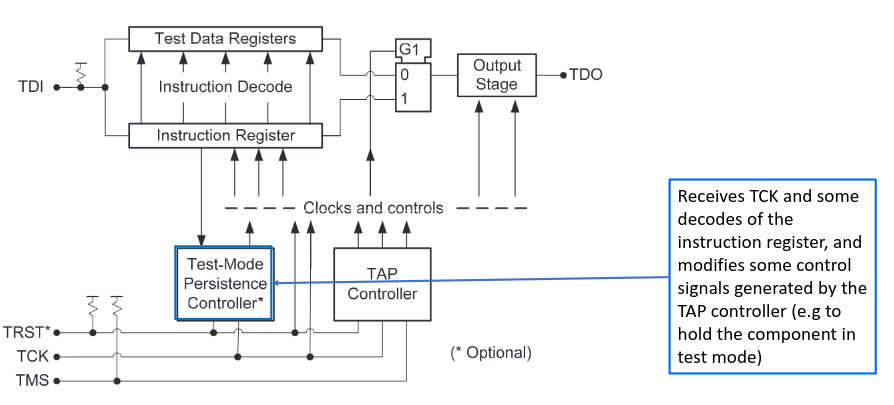
\includegraphics[width=0.7\textwidth]{img/hardware/tap scheme.png}
        \caption{The TAP scheme}
      \end{figure}

      The FSM is a 16 state machine, divided into 2 main branches: the data column and the
      instruction column. The data column is used to shift data in and out of the device, whilst the 
      instruction column is used to execute instructions. 
      \begin{figure}[H]
        \centering
        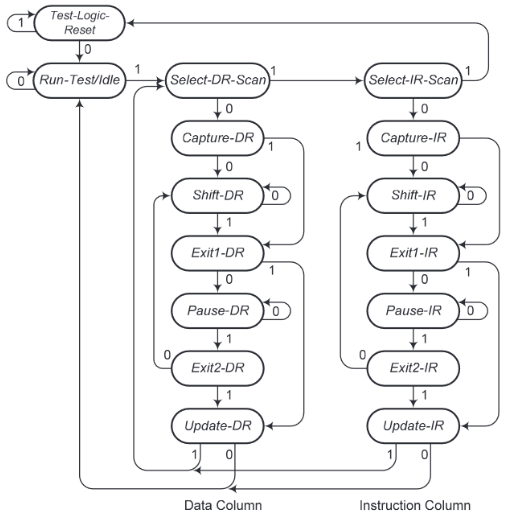
\includegraphics[width=0.5\textwidth]{img/hardware/tap fsm.png}
        \caption{The TAP FSM}
      \end{figure}
      In JTAP protocol, some instructions are mandatory and defined by the standard, while other are
      user defined. Some of the mandatory instructions are BYPASS(connects the TDI to the TDO),
      IDCODE, and SAMPLE/PRELOAD(connects the boundary scan register to the TDI and TDO).\\
      In particular the last instruction implies than its mandatory to give the possibility to get
      the content of the scan register, which can be used to leak informations. To avoid this, some
      strengthening of the protocol is needed, such as encryption and authentication mechanisms.
      Another possibility is to design resistance to probing, but this makes the board more
      expensive.\\
      Some other alternaves are to use obfuscation techniques. One example of this is to use a
      permutation network, which makes the logical connections between the components more complex.
      By making it random, we can design a mechanism in which the connection are the correct ones
      only if the correct key is provided. 
      \begin{figure}[H]
        \centering
        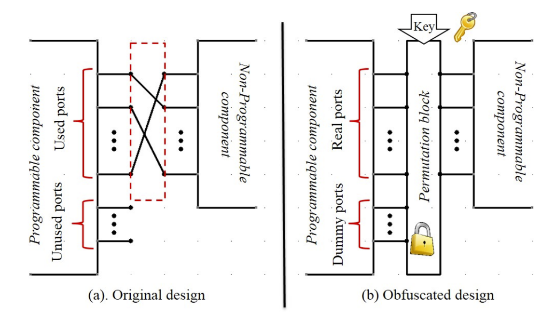
\includegraphics[width=0.5\textwidth]{img/hardware/permutation network.png}
        \caption{Permutation network}
      \end{figure}
      Another approach, which is more expensive to implement, is to use dummy integrated circuits,
      to obfuscate the real ones. 

    \end{subsubsection}

  \end{subsection}

\end{section}
